\documentclass[conference,10pt]{IEEEtran}
\IEEEoverridecommandlockouts
\usepackage[T1]{fontenc}
\usepackage{amsmath,amssymb}
\usepackage{graphicx}
\usepackage{booktabs}
\usepackage{xcolor}
\usepackage[hidelinks]{hyperref}
\usepackage{microtype}
\usepackage{cite}
\usepackage[font=footnotesize,skip=3pt]{caption}
\graphicspath{{figures/}}
% generated by scripts/report_numbers.py -- do not edit
\newcommand{\NumEpisodes}{512}
\newcommand{\NumSeeds}{3}
\newcommand{\GainLUT}{2.53}
\newcommand{\GainPPO}{2.92}
\newcommand{\GainPPOstd}{0.005}
\newcommand{\GainPPOoverLUT}{15}
\newcommand{\TravelGreedy}{143}
\newcommand{\TravelLUT}{290}
\newcommand{\TravelPPO}{147}
\newcommand{\TravelCutVsLUT}{49}
\newcommand{\PowerGreedy}{20.13}
\newcommand{\GainRandomAbs}{2.68}
\newcommand{\SwitchLUT}{2.2}
\newcommand{\GainLUTf}{2.72}
\newcommand{\TravelLUTf}{185}
\newcommand{\RewardLUTf}{1.04}
\newcommand{\RewardLUT}{0.87}
\newcommand{\RewardPPO}{1.15}
\newcommand{\AlphaLUTf}{0.6}
\newcommand{\SwitchPPO}{1.3}
\newcommand{\BetterEpisodesPPO}{99}
\newcommand{\SSoptimal}{5.40}
\newcommand{\SSppo}{5.27}
\newcommand{\SSfraction}{97}
\newcommand{\DecisionPPO}{0.10}
\newcommand{\DecisionSR}{888}
\newcommand{\ValLUT}{2.29}
\newcommand{\PairedLUTDiff}{0.39}
\newcommand{\PairedLUTSEM}{0.026}
\newcommand{\PairedLUTBetter}{84}
\newcommand{\PairedLUTfDiff}{0.19}
\newcommand{\PairedLUTfSEM}{0.017}
\newcommand{\PairedLUTfBetter}{72}
\newcommand{\HystLUT}{1.8}
\newcommand{\HystPPO}{5.3}
\newcommand{\HystPPOfwd}{272.7}
\newcommand{\HystPPObwd}{267.4}
\newcommand{\NoiseLUTZero}{3.39}
\newcommand{\NoiseLUTfZero}{3.07}
\newcommand{\NoisePPOZero}{3.05}
\newcommand{\NoiseLUTTwo}{2.55}
\newcommand{\NoiseLUTfTwo}{2.71}
\newcommand{\NoisePPOTwo}{2.93}
\newcommand{\NoiseLUTFour}{1.24}
\newcommand{\NoiseLUTfFour}{2.02}
\newcommand{\NoisePPOFour}{2.45}
\newcommand{\NoiseLUTSix}{0.38}
\newcommand{\NoiseLUTfSix}{1.40}
\newcommand{\NoisePPOSix}{1.83}
\newcommand{\MismatchGCHLUT}{2.73}
\newcommand{\MismatchGCHLUTf}{2.89}
\newcommand{\MismatchGCHPPO}{3.07}
\newcommand{\MismatchCCLUT}{3.05}
\newcommand{\MismatchCCLUTf}{3.22}
\newcommand{\MismatchCCPPO}{3.41}
\newcommand{\MismatchTILUT}{1.18}
\newcommand{\MismatchTILUTf}{1.25}
\newcommand{\MismatchTIPPO}{1.44}
\newcommand{\GammaMain}{0.5}
\newcommand{\ValRewardZero}{1.07}
\newcommand{\ValRewardPointEight}{1.01}
\newcommand{\ValRewardNinetyFive}{0.88}
\newcommand{\ValRewardHalf}{1.08}
\newcommand{\GammaZeroGain}{2.89}
\newcommand{\GammaZeroReward}{1.15}
\newcommand{\GammaHalfGain}{2.92}
\newcommand{\GammaHalfReward}{1.15}
\newcommand{\GammaPointEightGain}{2.79}
\newcommand{\GammaPointEightReward}{1.09}
\newcommand{\GammaNinetyFiveGain}{2.52}
\newcommand{\GammaNinetyFiveReward}{0.96}
\newcommand{\AblLongHorizonGain}{2.52}
\newcommand{\AblLongHorizonTravel}{169}
\newcommand{\AblLongHorizonReward}{0.96}
\newcommand{\AblNoSymmetryGain}{2.25}
\newcommand{\AblNoSymmetryTravel}{169}
\newcommand{\AblNoSymmetryReward}{0.84}
\newcommand{\AblNoPowersGain}{2.74}
\newcommand{\AblNoPowersTravel}{159}
\newcommand{\AblNoPowersReward}{1.07}
\newcommand{\AblNoYawCostGain}{2.92}
\newcommand{\AblNoYawCostTravel}{173}
\newcommand{\AblNoYawCostReward}{1.14}
   % generated by scripts/report_numbers.py
% Team members and repository link shown at the top of the report -- edit here.
\newcommand{\TeamMembers}{Rishi Agarwal (B23BB1036) \quad Abhishek Kumar (B23MT1003)}
\newcommand{\RepoURL}{https://github.com/Rishi-0312/AI-Assignment-2}
      % team members and repository URL

\newcommand{\wrap}{\operatorname{wrap}}
\setlength{\textfloatsep}{8pt plus 2pt minus 2pt}
\setlength{\floatsep}{6pt plus 2pt minus 2pt}
\setlength{\abovedisplayskip}{3pt}
\setlength{\belowdisplayskip}{3pt}

\begin{document}
\title{WakeSteer: Symmetry-Aware Deep Reinforcement\\Learning for Wind-Farm Wake Steering}
\author{\IEEEauthorblockN{\TeamMembers}
\IEEEauthorblockA{AI Course Mini-Project, Assignment 2 (Real-Life Use Cases of RL)\\
Code, trained agents \& reproduction: \url{\RepoURL}}}
\maketitle

\begin{abstract}
Wakes from upstream turbines cut the output of downstream machines by up to 75\% in the farm we study.
\emph{Wake steering} deliberately yaws upstream rotors away from the wind to deflect their wakes, but the
industrial practice---a look-up table (LUT) of set-points optimised offline with an engineering model---ignores
sensor noise, yaw-drive limits and actuator wear. We cast farm-level yaw control as a Markov decision process
with stochastic wind, noisy sensing, rate-limited yaw drives and a wear penalty, simulated with NREL's FLORIS,
and solve it with PPO (implemented from scratch) using an exactly rotation-equivariant policy. On \NumEpisodes{}
held-out one-hour episodes of a 3$\times$3 farm, the agent raises energy yield by \GainPPO\% over greedy
control, versus \GainLUT\% for a LUT optimised with the very same wake model, while yawing \TravelCutVsLUT\%
less than the LUT and deciding in \DecisionPPO\,ms instead of \DecisionSR\,ms.
\end{abstract}

\section{Introduction}
Wind farms lose 10--20\% of their energy to wake interactions. Yawing an upstream turbine by $\gamma$ costs it
roughly a $\cos^{1.88}\gamma$ fraction of its power but bends its wake away from downstream rotors, which can
recover far more~\cite{bastankhah2016,howland2019,fleming2019}. Choosing the yaw offsets of all turbines jointly
is a sequential decision problem: the wind direction drifts and is only measured noisily, yaw drives are slow,
and every degree of yaw travel wears the drive. Offline-optimised LUTs~\cite{fleming2022sr} treat each instant
in isolation and trust a perfect model and perfect measurements. Reinforcement learning (RL) instead optimises
closed-loop behaviour directly from interaction~\cite{stanfel2020,dong2021,kadoche2023}. Our contributions:
(i) a rigorous MDP of \emph{dynamic} wake steering with realistic sensing and actuation constraints;
(ii) a batched, Gymnasium-compatible FLORIS environment fast enough for on-policy RL on a laptop;
(iii) a PPO agent whose policy is exactly equivariant to the farm's 90$^\circ$ rotation symmetry; and
(iv) a paired, held-out evaluation against greedy and model-based control, with ablations and robustness tests.

\section{MDP Formulation}
\textbf{Farm and simulator.} Nine NREL 5-MW turbines~\cite{jonkman2009} ($D=126$\,m, $P_\mathrm{rated}=5$\,MW)
on a 3$\times$3 grid with $5D$ spacing, turbulence intensity 6\%. Turbine powers come from FLORIS~v4~\cite{floris}
with the Gauss--Curl-Hybrid wake model (Gaussian deficit, wake deflection, secondary steering and yaw-added
recovery~\cite{king2021}). One control step is $\Delta t=60$\,s; an episode is one hour ($T=60$).

\textbf{Exogenous wind.} The direction follows a persistent random walk $\theta_{t+1}=\theta_t+\delta_{t+1}$,
$\delta_{t+1}=0.7\,\delta_t+0.8^\circ\epsilon_t$; the speed is an Ornstein--Uhlenbeck process
$U_{t+1}=U_t+0.1(\bar U-U_t)+0.25\,\epsilon'_t$ with episode mean $\bar U\sim\mathcal U[5,12]$\,m/s and
$\theta_0\sim\mathcal U[0^\circ,360^\circ)$. Controllers only see 1-min measurements
$\hat\theta_t=\theta_t+\mathcal N(0,2^{\circ\,2})$, $\hat U_t=U_t+\mathcal N(0,0.2^2)$.

\textbf{State space $\mathcal S$.} The Markov state contains the true wind $(\theta,\delta,U,\bar U)$, the
measurements and the nacelle headings $h_i$. The agent observes $o_t\in\mathbb R^{22}$ (a POMDP):
\begin{equation*}
o_t=\Big[\sin\hat\theta_t,\ \cos\hat\theta_t,\ \tfrac{\hat U_t-8.5}{3.5},\ \tfrac{\Delta\hat\theta_t}{5^\circ},\
\big\{\tfrac{\hat\gamma_{i,t}}{25^\circ}\big\}_{i=1}^{9},\ \big\{\tfrac{P_{i,t}}{P_\mathrm{rated}}\big\}_{i=1}^{9}\Big],
\end{equation*}
with $\hat\gamma_i=\wrap(\hat\theta-h_i)$ the measured yaw offsets and $P_i$ the turbine outputs. The outputs
depend on the \emph{true} wind, so they act as an implicit, noise-free wake sensor.

\textbf{Action space $\mathcal A$.} Continuous $a_t\in[-1,1]^9$: yaw-offset set-points $\gamma^\star_i=25^\circ a_i$.
The yaw drives turn each nacelle towards $\hat\theta_t-\gamma^\star_i$ at most $\omega=0.3^\circ$/s:
$h_{i,t+1}=h_{i,t}+\Delta h_{i,t}$, $\Delta h_{i,t}=\mathrm{clip}\big(\wrap(\hat\theta_t-\gamma^\star_i-h_{i,t}),\pm\omega\Delta t\big)$.
The wind then evolves and FLORIS returns $P_{i,t+1}$ for the true misalignments $\gamma_i=\theta_{t+1}-h_{i,t+1}$.

\textbf{Reward $\mathcal R$} (in \% of farm capacity $P_\mathrm{cap}=45$\,MW):
\begin{equation}
r_t=\frac{100}{P_\mathrm{cap}}\Big(\sum_{i}P_{i,t+1}-P^\mathrm{greedy}(\theta_{t+1},U_{t+1})\Big)-c\sum_i|\Delta h_{i,t}|.
\label{eq:reward}
\end{equation}
$P^\mathrm{greedy}$ is the power of the all-aligned farm in the same wind (tabulated once). Because no controller
can influence the wind, this term shifts every policy's return by the same amount: the optimal policy is
unchanged, but the large reward variance caused by the $U^3$ power law disappears. The second term
($c=0.005$ per degree) prices yaw-drive wear and discourages chattering.

\section{Environment, Algorithm and Baselines}
\textbf{Fast environment.} A FLORIS call costs $\approx$20\,ms of fixed overhead, so all 256 parallel
environments are advanced in lock-step with \emph{one} vectorised FLORIS evaluation per step, split across worker
processes ($\approx$3.8k env-steps/s on an i7-12700H). The same dynamics are exposed as a Gymnasium
environment (\texttt{WakeSteer-v0}).

\textbf{Symmetry-aware policy.} The grid is invariant under 90$^\circ$ rotation and FLORIS works in the wind
frame, so $P_i(\theta,\boldsymbol\gamma)=P_{\pi(i)}(\theta-90^\circ,\Pi\boldsymbol\gamma)$ for a fixed turbine
permutation $\pi$ (verified to $10^{-6}$). Before the networks, each observation is rotated by $k$ quarter
turns into the canonical sector $\hat\theta-90^\circ k\in[15^\circ,105^\circ)$ (cut where steering gains vanish)
with turbine features permuted by $\pi^k$; the actions are permuted back. The policy is thus equivariant by
construction and only needs to learn a quarter of the wind rose.

\textbf{PPO~\cite{schulman2017}.} Gaussian policy with state-independent std; actor and critic are separate
2$\times$256 tanh MLPs whose direction input is expanded into Fourier features $\sin k\theta,\cos k\theta$,
$k\in\{1,2,3,4,8\}$. Clipped surrogate ($\epsilon=0.2$), GAE~\cite{schulman2016} ($\gamma=0.95$, $\lambda=0.9$),
256 envs$\times$30 steps per update, 10 epochs of 8 minibatches, Adam ($3\!\times\!10^{-4}$, linearly annealed),
early stop at KL$>$0.02, per-network gradient clipping, and bootstrapping at time-limit truncations.
Training starts from random yaw offsets (exploring starts) and runs $5\times10^6$ steps ($\approx$70\,min);
the checkpoint with the best return on fixed validation weather is kept. PPO suits the problem: actions are
continuous and 9-dimensional (a discretised DQN would need $\gg10^8$ joint actions) and on-policy updates are
stable while simulated experience is cheap.

\textbf{Baselines.} \emph{Greedy}: zero offsets---every turbine tracks the measured wind (industry standard).
\emph{LUT}: offsets optimised offline by FLORIS' Serial-Refine method~\cite{fleming2022sr} on a
$1^\circ\times1$\,m/s grid with the \emph{same} wake model the agent trains in (3\,960 optimisations), looked up at
the measured wind---a strong model-based reference with perfect model knowledge. \emph{Random} set-points.
All controllers share the yaw dynamics and are tested on \NumEpisodes{} one-hour episodes whose weather was
never seen in training or validation; each controller faces \emph{identical} wind realisations.

\section{Results}
\begin{table}[t]
\centering
\caption{Held-out test: \NumEpisodes{} one-hour episodes, identical weather for every controller.}
\label{tab:main}
\setlength{\tabcolsep}{3.2pt}
\footnotesize
\begin{tabular}{@{}lrrrr@{}}
\toprule
Controller & Power & Energy gain & Yaw travel & Reward\\
 & [MW] & vs greedy [\%] & [$^\circ$/turb./h] & per step\\
\midrule
% generated by scripts/report_numbers.py -- do not edit
Greedy (baseline) & +0.00 & 143 & 0.4 & \textminus{}0.15 \\
LUT (FLORIS-SR) & +2.53 & 290 & 2.2 & +0.87 \\
LUT + filter ($\alpha$=0.6) & +2.72 & 185 & 1.4 & +1.04 \\
\midrule
\textbf{PPO (ours, 3 seeds)} & \textbf{+2.92$\pm$0.005} & \textbf{147$\pm$2} & \textbf{1.3} & \textbf{+1.15} \\
\ -- long horizon ($\gamma$\,=\,0.95) & +2.52 & 169 & 1.5 & +0.96 \\
\ -- plain MLP ($\gamma$\,=\,0.95) & +2.25 & 169 & 1.7 & +0.84 \\
\ -- no power inputs & +2.74 & 159 & 1.4 & +1.07 \\
\ -- no wear penalty & +2.92 & 173 & 1.4 & +1.14 \\
\bottomrule

\bottomrule
\end{tabular}
\end{table}

\begin{figure}[t]
\centering
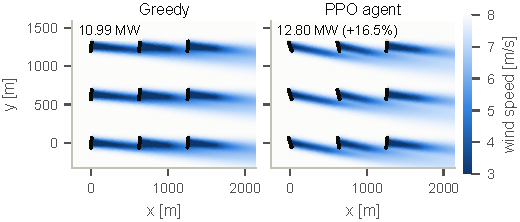
\includegraphics[width=\columnwidth]{fig_flow}
\caption{Hub-height flow at $270^\circ$, 8\,m/s: greedy control versus the settled PPO set-points, which
deflect the upstream wakes off the downstream rotors.}
\label{fig:flow}
\end{figure}

\textbf{Main result.} Table~\ref{tab:main}: PPO gains \GainPPO$\pm$\GainPPOstd\% energy over greedy control
(mean$\pm$std over \NumSeeds{} seeds; better than greedy in \BetterEpisodesPPO\% of episodes), against
\GainLUT\% for the LUT, while yawing \TravelPPO$^\circ$ per turbine-hour instead of \TravelLUT$^\circ$. The LUT
reacts to every noisy direction measurement, flipping offsets back and forth near turbine alignments; the agent
has learned to filter the noise, to read the true wake situation from the turbine outputs and to hold a
deflection side (hysteresis) unless switching pays off over the coming minutes. Fig.~\ref{fig:flow} shows the
resulting wake deflection.

\begin{figure}[t]
\centering
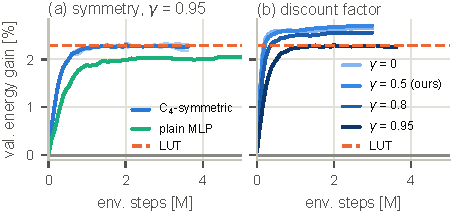
\includegraphics[width=\columnwidth]{fig_training}
\caption{Validation energy gain during training. The symmetric policy learns much faster than a plain MLP.}
\label{fig:training}
\end{figure}

\begin{figure}[t]
\centering
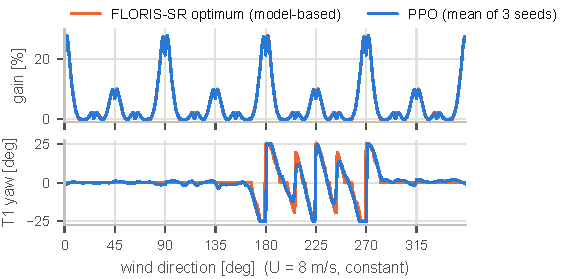
\includegraphics[width=\columnwidth]{fig_sweep}
\caption{Steady state (constant, noise-free wind). Top: farm power gain over greedy. Bottom: yaw offset of
corner turbine T1; the learned schedule reproduces the model-optimal sign switches at turbine alignments.}
\label{fig:sweep}
\end{figure}

\textbf{Learning and ablations.} The C$_4$-equivariant policy learns markedly faster than a plain MLP
(Fig.~\ref{fig:training}; \AblNoSymmetryGain\% after the same budget). A myopic agent ($\gamma=0$, i.e.\ a
contextual bandit) reaches \AblMyopicGain\%, confirming that the sequential formulation matters. Without the
turbine-power inputs the gain drops to \AblNoPowersGain\%, and removing the wear penalty raises yaw travel to
\AblNoYawCostTravel$^\circ$/h.

\textbf{What was learned.} In constant, noise-free wind (Fig.~\ref{fig:sweep}) the agent recovers
\SSfraction\% of the model-optimal steady-state gain (\SSppo\% vs \SSoptimal\% at 8\,m/s) without ever being
told the optimum, including the discontinuous sign switches of the optimal yaw schedule.

\begin{figure}[t]
\centering
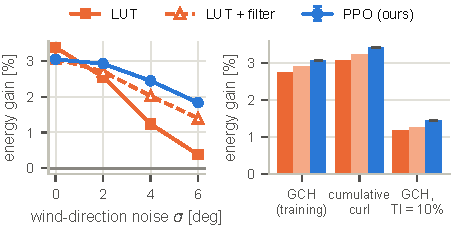
\includegraphics[width=\columnwidth]{fig_robustness}
\caption{Robustness without retraining. Left: wind-direction measurement noise. Right: wake-model and
turbulence mismatch (both controllers were built with GCH at TI\,=\,6\%).}
\label{fig:robust}
\end{figure}

\textbf{Robustness.} With perfect direction measurements the LUT is near-optimal (\NoiseLUTZero\% vs
\NoisePPOZero\%), but its gain collapses as noise grows (\NoiseLUTSix\% at $\sigma=6^\circ$) while the agent
keeps \NoisePPOSix\% (Fig.~\ref{fig:robust}). Under a different wake model (cumulative curl) both controllers
remain profitable (LUT \MismatchCCLUT\%, PPO \MismatchCCPPO\%), and at TI\,=\,10\% gains shrink for both
(\MismatchTILUT\% vs \MismatchTIPPO\%).

\section{Conclusion}
A PPO agent trained in FLORIS learns wake-steering yaw control that beats both greedy control and a
model-optimised look-up table under realistic sensing and actuation, at a fraction of the yaw activity and with
microsecond-scale decisions. Encoding the farm's rotation symmetry in the policy was the key to sample
efficiency. Limitations: a steady-state wake model (no wake advection delay), a single layout and simulated
sensors; next steps are dynamic wake models, layout-agnostic graph policies and field data.

\begin{thebibliography}{10}
\footnotesize
\bibitem{floris} NREL, ``FLORIS: FLOw Redirection and Induction in Steady State, v4,'' 2024. \url{https://github.com/NREL/floris}
\bibitem{bastankhah2016} M.~Bastankhah and F.~Port\'e-Agel, ``Experimental and theoretical study of wind turbine wakes in yawed conditions,'' \emph{J. Fluid Mech.}, vol.~806, pp.~506--541, 2016.
\bibitem{king2021} J.~King \emph{et al.}, ``Control-oriented model for secondary effects of wake steering,'' \emph{Wind Energy Science}, vol.~6, pp.~701--714, 2021.
\bibitem{fleming2022sr} P.~Fleming \emph{et al.}, ``Serial-refine method for fast wake-steering yaw optimization,'' \emph{J. Phys.: Conf. Ser.}, vol.~2265, 032109, 2022.
\bibitem{howland2019} M.~F.~Howland, S.~K.~Lele and J.~O.~Dabiri, ``Wind farm power optimization through wake steering,'' \emph{PNAS}, vol.~116, no.~29, pp.~14495--14500, 2019.
\bibitem{fleming2019} P.~Fleming \emph{et al.}, ``Initial results from a field campaign of wake steering applied at a commercial wind farm -- Part 1,'' \emph{Wind Energy Science}, vol.~4, pp.~273--285, 2019.
\bibitem{jonkman2009} J.~Jonkman, S.~Butterfield, W.~Musial and G.~Scott, ``Definition of a 5-MW reference wind turbine for offshore system development,'' NREL/TP-500-38060, 2009.
\bibitem{schulman2017} J.~Schulman, F.~Wolski, P.~Dhariwal, A.~Radford and O.~Klimov, ``Proximal policy optimization algorithms,'' arXiv:1707.06347, 2017.
\bibitem{schulman2016} J.~Schulman, P.~Moritz, S.~Levine, M.~Jordan and P.~Abbeel, ``High-dimensional continuous control using generalized advantage estimation,'' in \emph{Proc. ICLR}, 2016.
\bibitem{stanfel2020} P.~Stanfel, K.~Johnson, C.~J.~Bay and J.~King, ``A distributed reinforcement learning yaw control approach for wind farm energy capture maximization,'' in \emph{Proc. American Control Conf.}, 2020, pp.~4065--4070.
\bibitem{dong2021} H.~Dong, J.~Zhang and X.~Zhao, ``Intelligent wind farm control via deep reinforcement learning and high-fidelity simulations,'' \emph{Applied Energy}, vol.~292, 116928, 2021.
\bibitem{kadoche2023} E.~Kadoche, S.~Gourv\'enec, M.~Pallud and T.~Levent, ``MARLYC: Multi-agent reinforcement learning yaw control,'' \emph{Renewable Energy}, vol.~217, 119129, 2023.
\end{thebibliography}
\end{document}
